\begin{figure}[!h]
  \begin{center}
    \caption{Illustration des différents vecteurs introduits}%
    \label{vis:ill}
    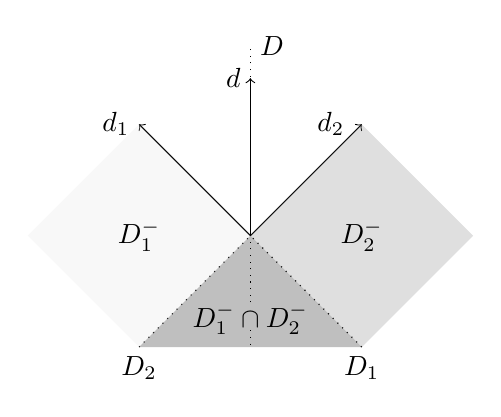
\begin{tikzpicture}
      \begin{scope}[rotate=45]
        \draw [<-] (2, 0) node[left] {$d_2$\phantom{i}} -- (0, 0);
        \draw [dotted] (-2, 0) node[below] {$D_2$} -- (0, 0);
        \draw [->] (0, 0)-- (0, 2) node[left] {$d_1$};
        \draw [dotted] (0, -2) node[below] {$D_1$} -- (0, 0);
        \draw [->] (0, 0) -- (1.41421, 1.41421) node[left] {$d$};
        \fill [black!50, nearly transparent](0, 0) -- (2, 0) -- (2, -2)%
        -- (0, -2) -- cycle;
        \fill [black!10, nearly transparent](0, 0) -- (-2, 0) -- (-2, 2)%
        -- (0, 2) -- cycle;
        \fill [black, nearly transparent] (0, 0) -- (0, -2) -- (-2, 0) -- cycle;
        \draw (-1, 1) node{$D_1^-$};
        \draw (1, -1) node{$D_2^-$};
        \draw (-0.75, -0.75) node {$D_1^-\cap D^-_2$};
        \draw [dotted] (-0.6, -0.6)  -- (1.7, 1.7) node[right] {$D$};
        \draw [dotted] (-0.85, -0.85)  -- (-1, -1);
      \end{scope}
    \end{tikzpicture}
\end{center}
\end{figure}
%%% Local Variables:
%%% mode: latex
%%% TeX-master: "../rapportGp1"
%%% End:
